\appendix
\chapter{Curve di discriminazione}                          %imposta le appendici
Vengono di seguito riportate le curve di discriminazione dei vari fotomoltiplicatori del iani di rivelazione 0 e 1.

\begin{figure}[H]
	\centering
	\subfloat[][]{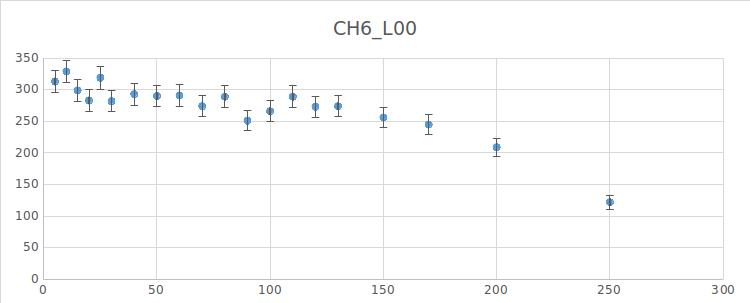
\includegraphics[width=.6\textwidth]{excel-plots/disc-L00.jpg}\label{fig:disc-L00}}\quad
	\subfloat[][]{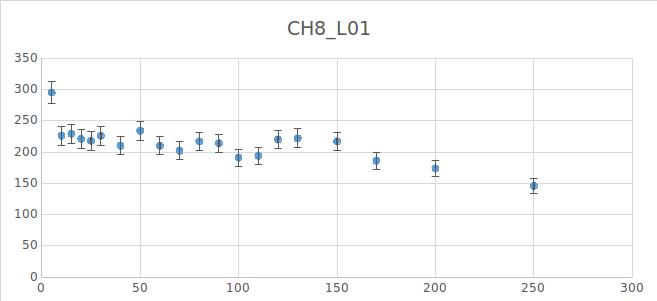
\includegraphics[width=.6\textwidth]{excel-plots/disc-L01.jpg}\label{fig:disc-L01}}\quad
	\subfloat[][]{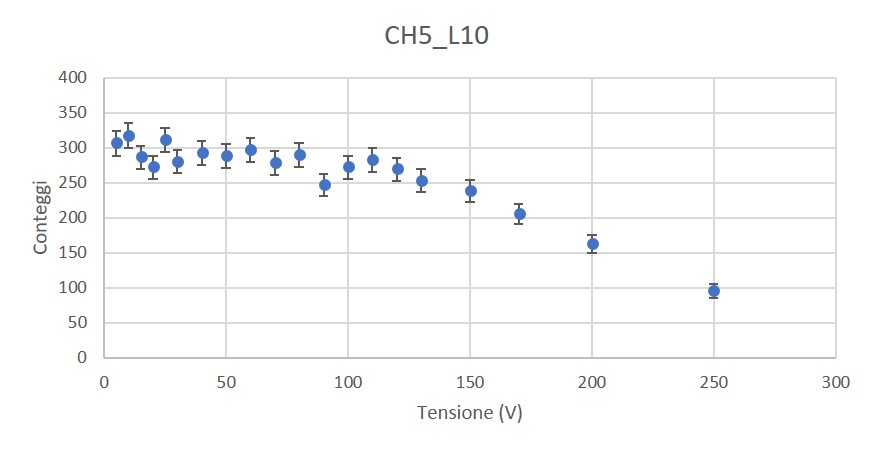
\includegraphics[width=.6\textwidth]{excel-plots/disc-L10.jpg}\label{fig:disc-L10}}\quad
	\subfloat[][]{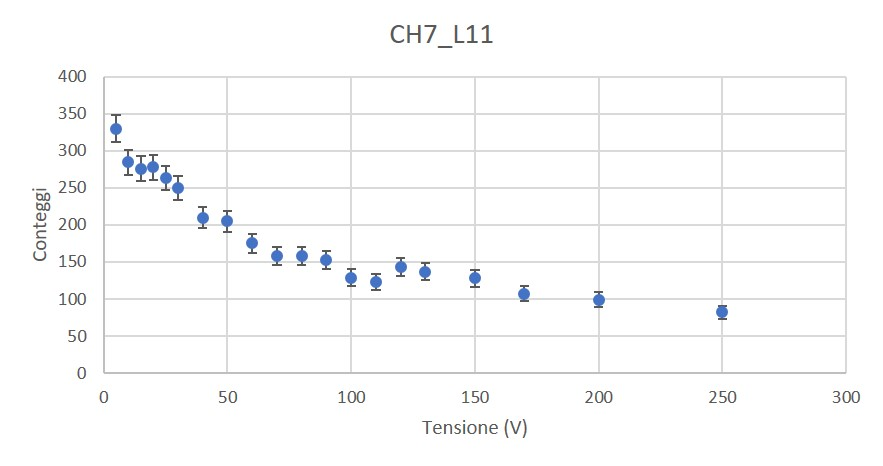
\includegraphics[width=.6\textwidth]{excel-plots/disc-L11.jpg}\label{fig:disc-L11}}\quad
\end{figure}
\begin{figure}[H]
	\centering
	\subfloat[][]{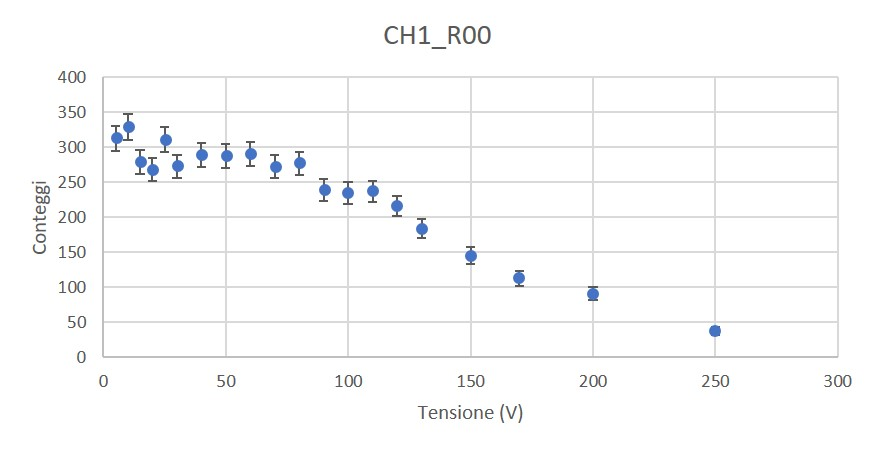
\includegraphics[width=.6\textwidth]{excel-plots/disc-R00.jpg}\label{fig:disc-R00}}\quad
	\subfloat[][]{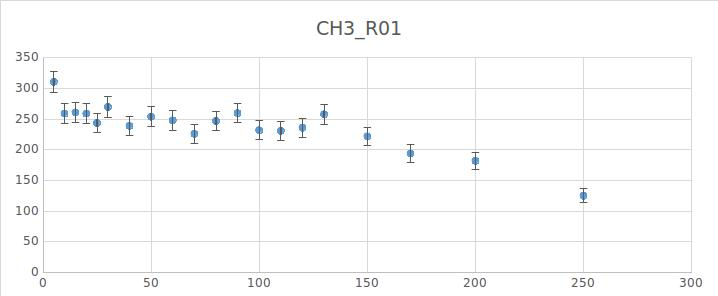
\includegraphics[width=.6\textwidth]{excel-plots/disc-R01.jpg}\label{fig:disc-R01}}\quad
	\subfloat[][]{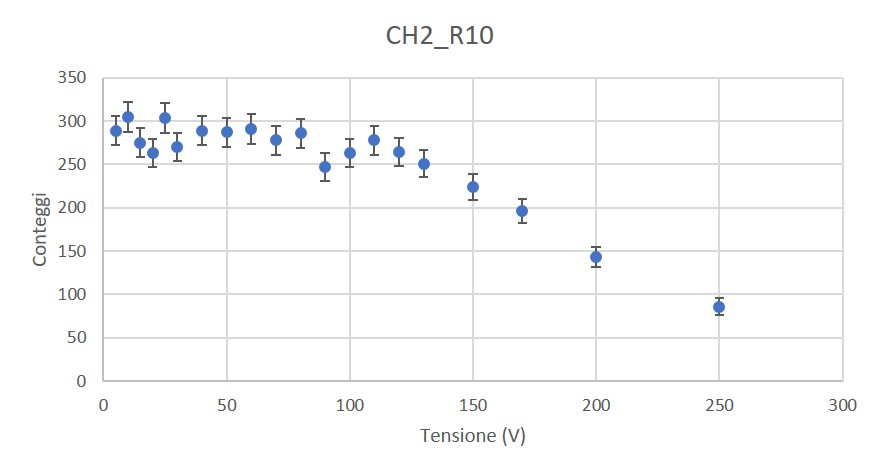
\includegraphics[width=.6\textwidth]{excel-plots/disc-R10.jpg}\label{fig:disc-R10}}\quad
	\subfloat[][]{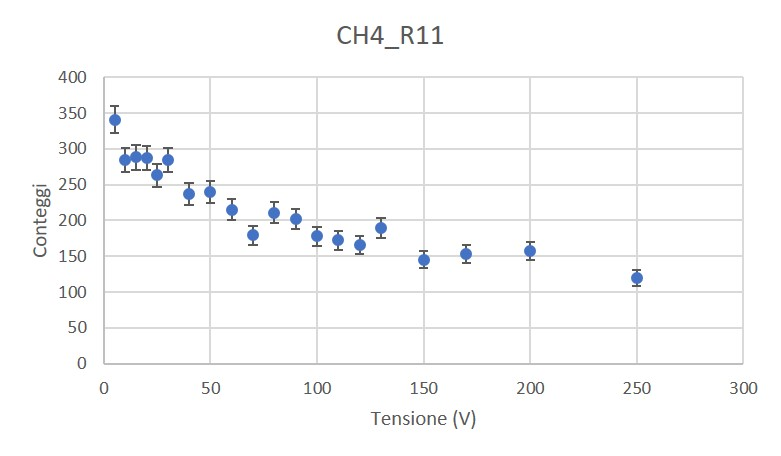
\includegraphics[width=.6\textwidth]{excel-plots/disc-R11.jpg}\label{fig:disc-R11}}\quad
\end{figure}
\chapter{Rette di calibrazione dei TDC}               %crea l'appendice
Vengono di seguito riportate le rette di calibrazione del Time to Digital Converter.

\begin{figure}[H]
  \centering
  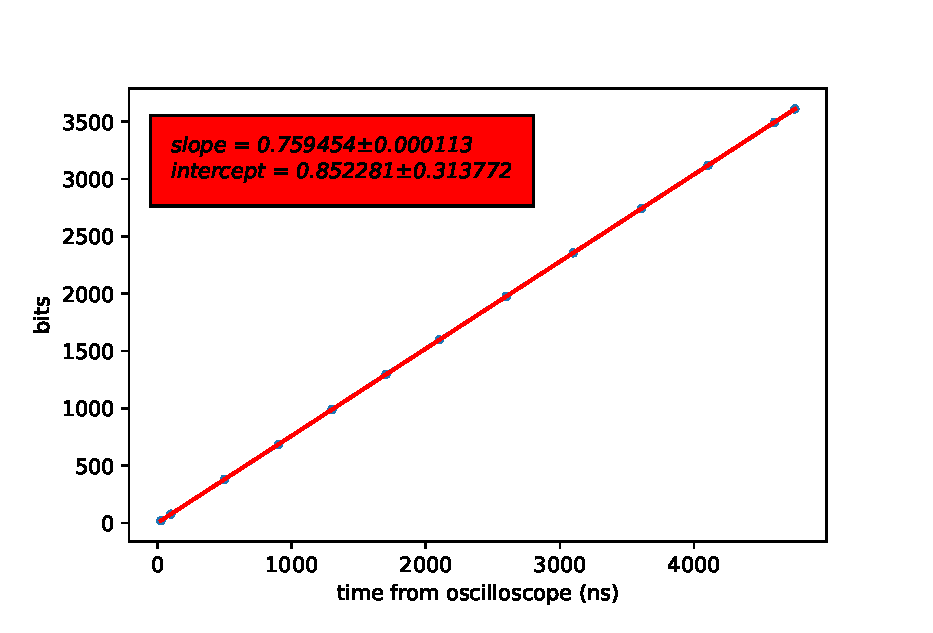
\includegraphics[width=.8\textwidth]{plots/tdc11.eps}
  \caption{Retta di calibrazione del canale 1 del TDC 1.}
  \label{fig:tdc11}
\end{figure}

\begin{figure}[H]
  \centering
  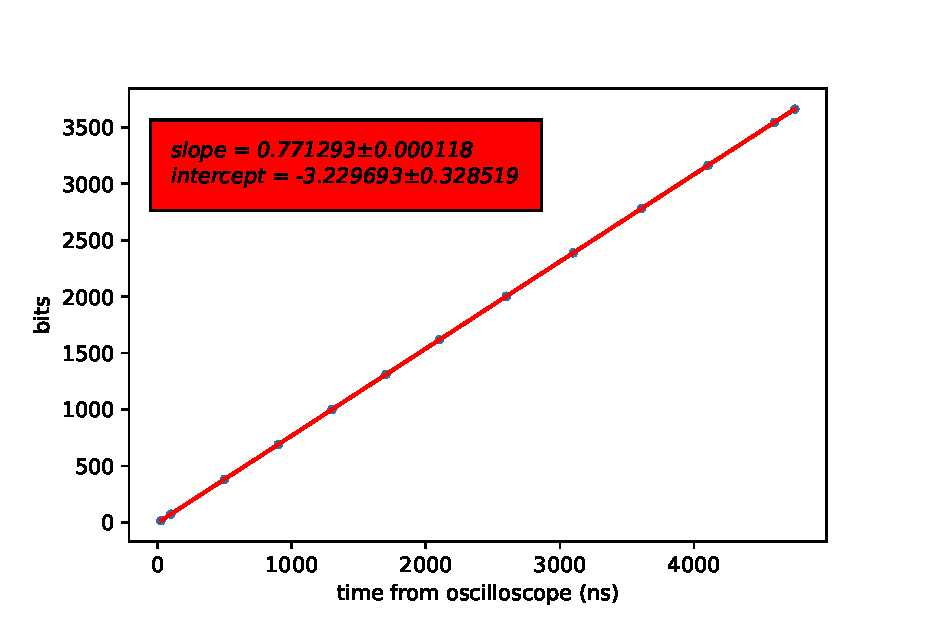
\includegraphics[width=.8\textwidth]{plots/tdc12.eps}
  \caption{Retta di calibrazione del canale 2 del TDC 1.}
  \label{fig:tdc12}
\end{figure}

\begin{figure}[H]
  \centering
  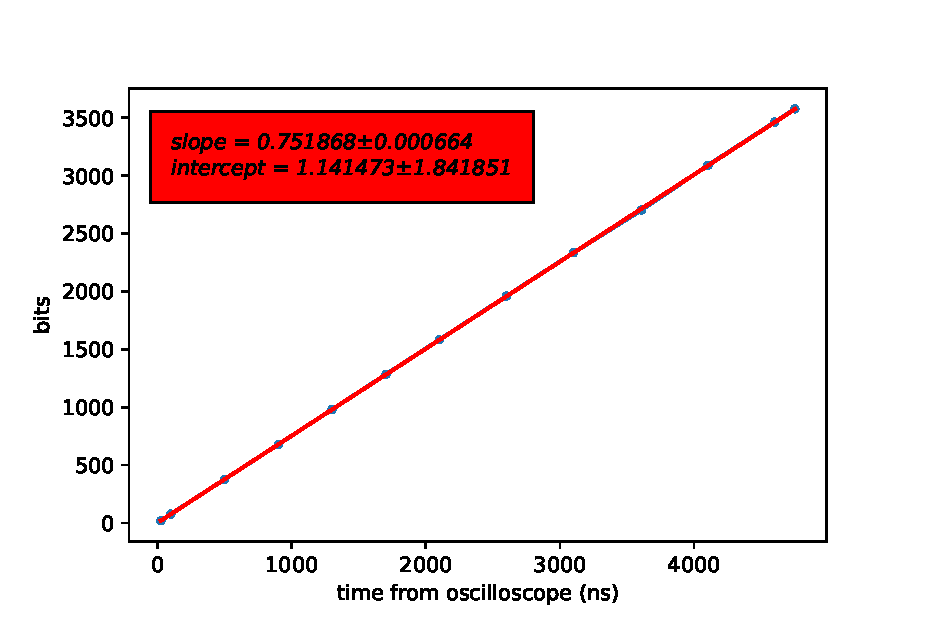
\includegraphics[width=.8\textwidth]{plots/tdc13.eps}
  \caption{Retta di calibrazione del canale 3 del TDC 1.}
  \label{fig:tdc13}
\end{figure}

\begin{figure}[H]
  \centering
  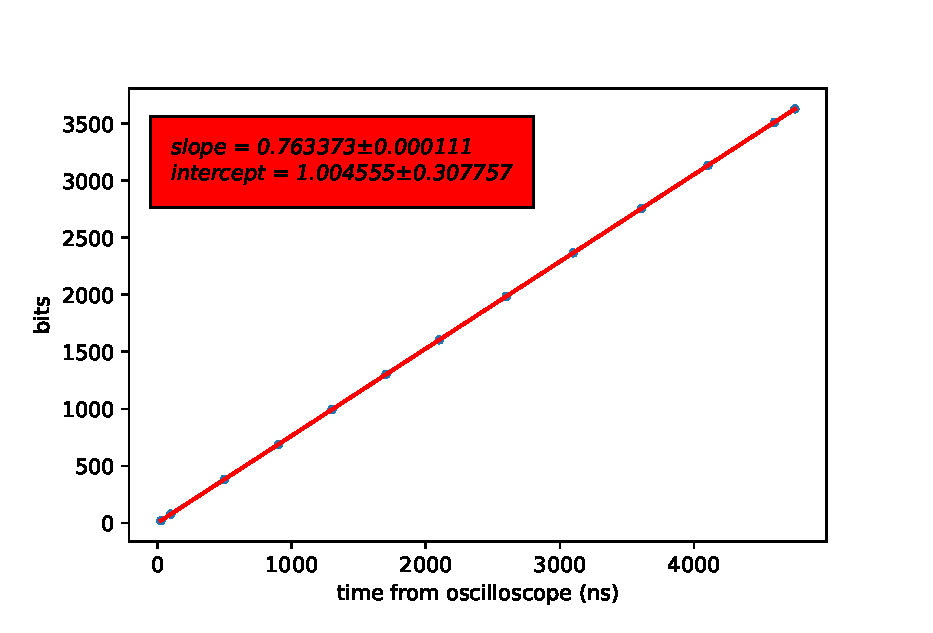
\includegraphics[width=.8\textwidth]{plots/tdc14.eps}
  \caption{Retta di calibrazione del canale 4 del TDC 1.}
  \label{fig:tdc14}
\end{figure}

\begin{figure}[H]
  \centering
  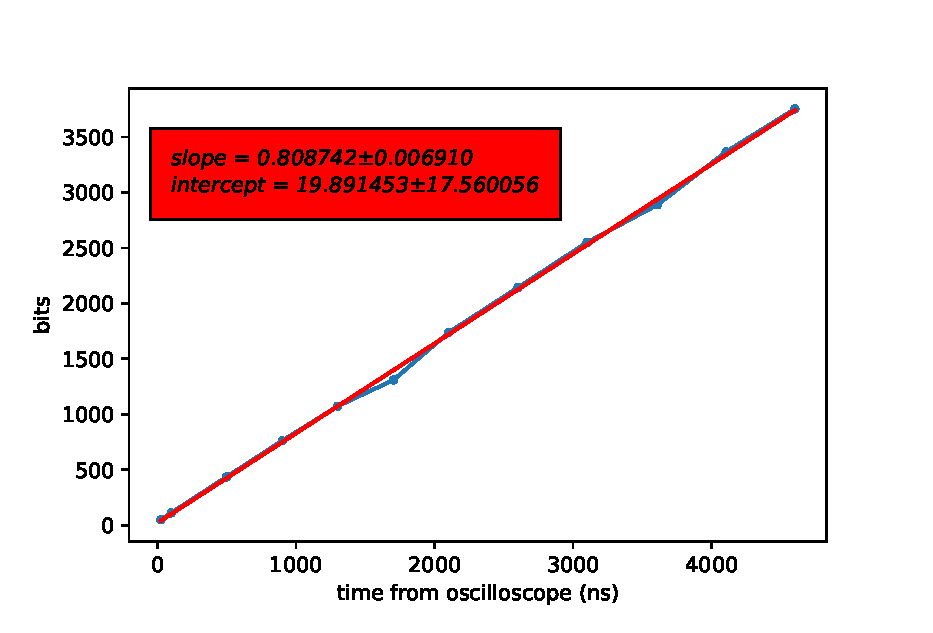
\includegraphics[width=.8\textwidth]{plots/tdc23.eps}
  \caption{Retta di calibrazione del canale 3 del TDC 2.}
  \label{fig:tdc23}
\end{figure}

\begin{figure}[H]
  \centering
  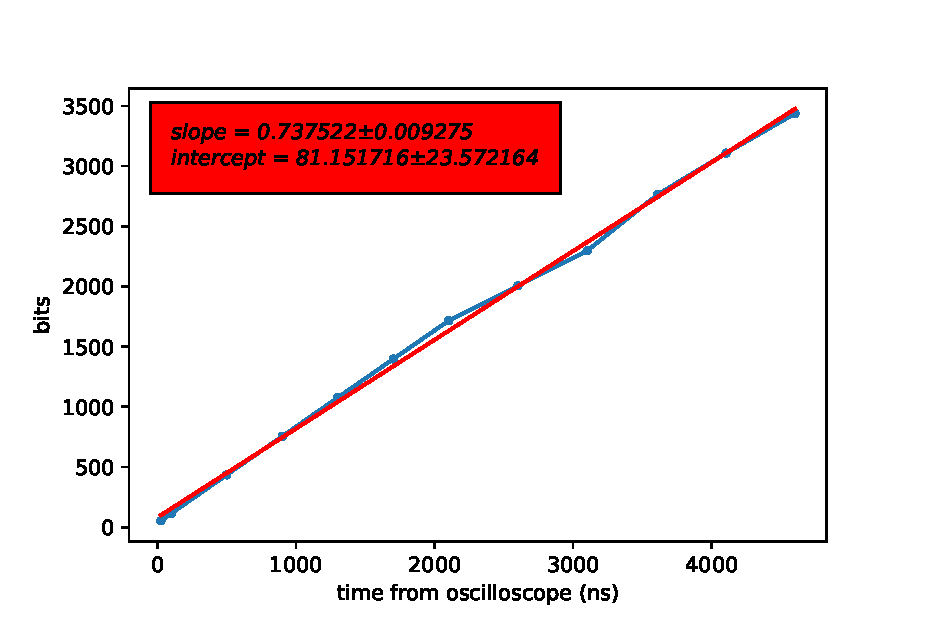
\includegraphics[width=.8\textwidth]{plots/tdc24.eps}
  \caption{Retta di calibrazione del canale 4 del TDC 2.}
  \label{fig:tdc24}
\end{figure}

\begin{figure}[H]
  \centering
  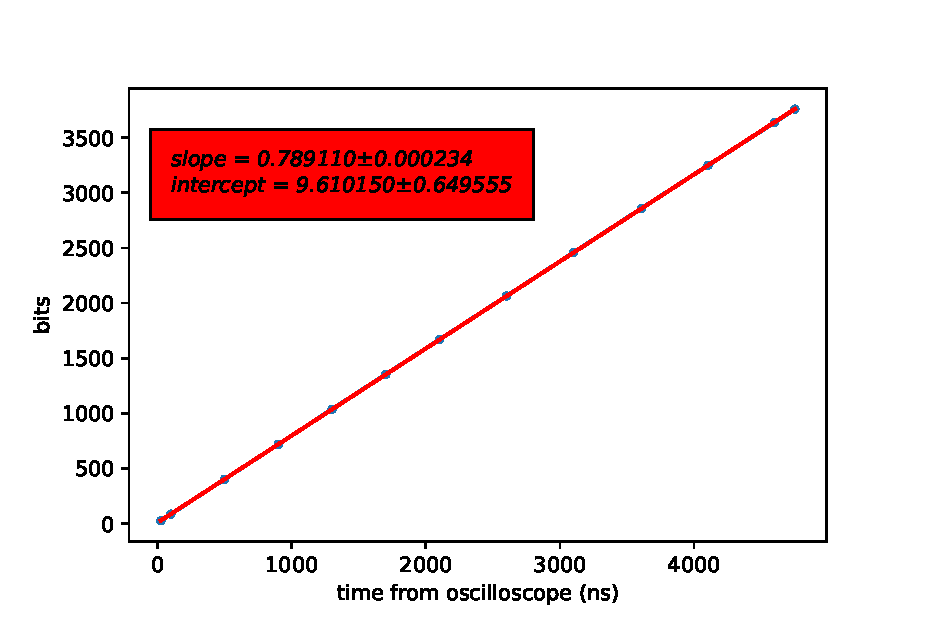
\includegraphics[width=.8\textwidth]{plots/tdc25.eps}
  \caption{Retta di calibrazione del canale 2 del TDC 5.}
  \label{fig:tdc25}
\end{figure}

\begin{figure}[H]
  \centering
  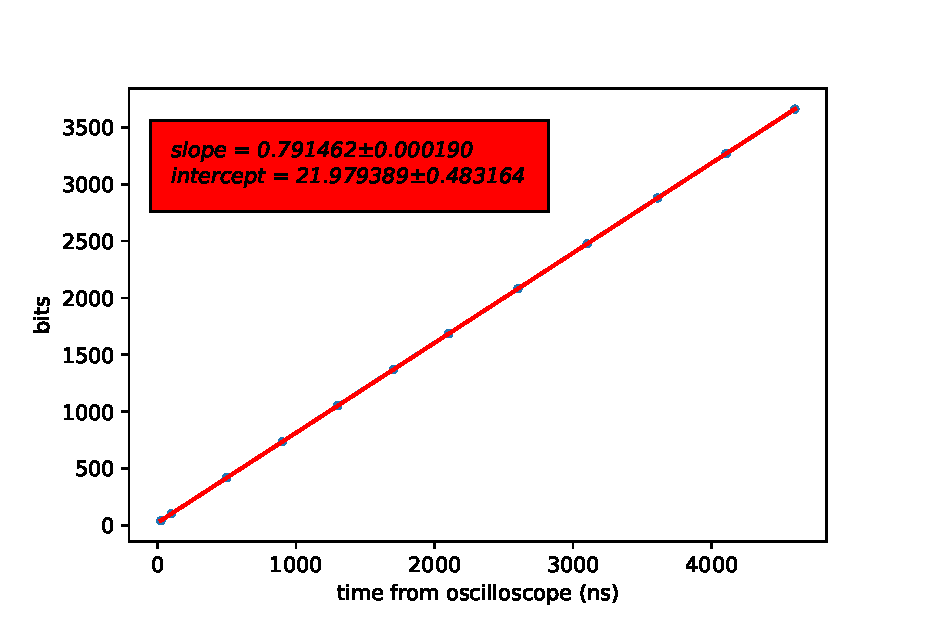
\includegraphics[width=.8\textwidth]{plots/tdc26.eps}
  \caption{Retta di calibrazione del canale 6 del TDC 2.}
  \label{fig:tdc26}
\end{figure}



%\rhead[\fancyplain{}{\bfseries \thechapter \:Prima Appendice}]
%{\fancyplain{}{\bfseries\thepage}}

\chapter{Perdita di Energia}             %crea l'appendice
%%%%%%%%%%%%%%%%%%%%%%%%%%%%%%%%%%%%%%%%%imposta l'intestazione di pagina
%\rhead[\fancyplain{}{\bfseries \thechapter \:Seconda Appendice}]
%{\fancyplain{}{\bfseries\thepage}}
Si riportano le distribuzioni della perdita di energia per i vari semipiani, completi della distribuzioni di Landau che rappresentano il best fit.

\begin{figure}[H]
  \centering
  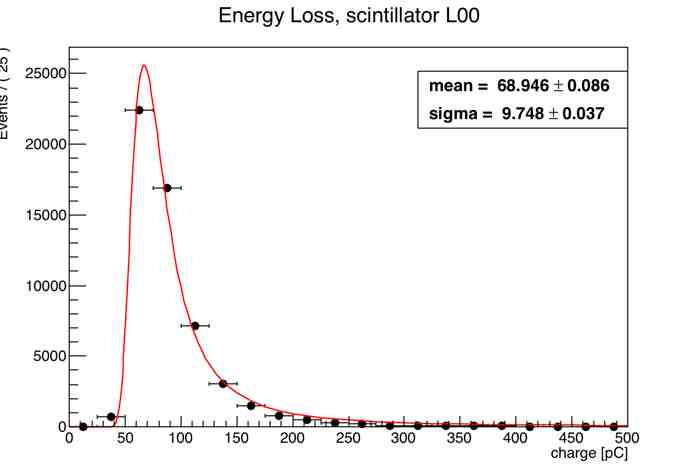
\includegraphics[width=0.8\textwidth]{plots/energy_L00.jpg}
  \caption{Curva della perdita di energia per il piano L00.}
  \label{fig:l00}
\end{figure}

\begin{figure}[H]
  \centering
  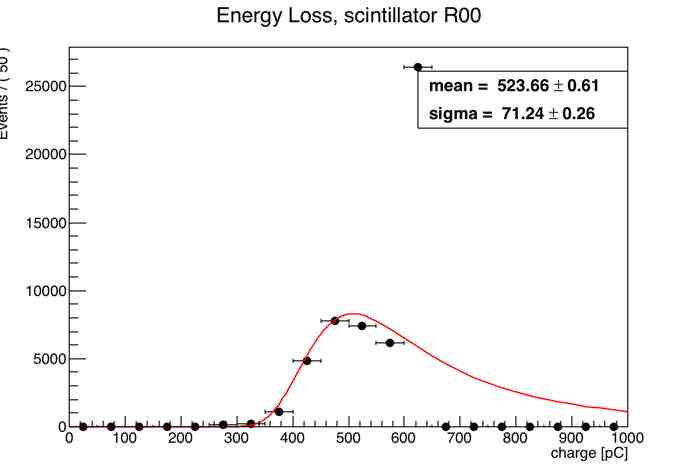
\includegraphics[width=0.8\textwidth]{plots/energy_R00.jpg}
  \caption{Curva della perdita di energia per il piano R00.}
  \label{fig:r00}
\end{figure}

\begin{figure}[H]
  \centering
  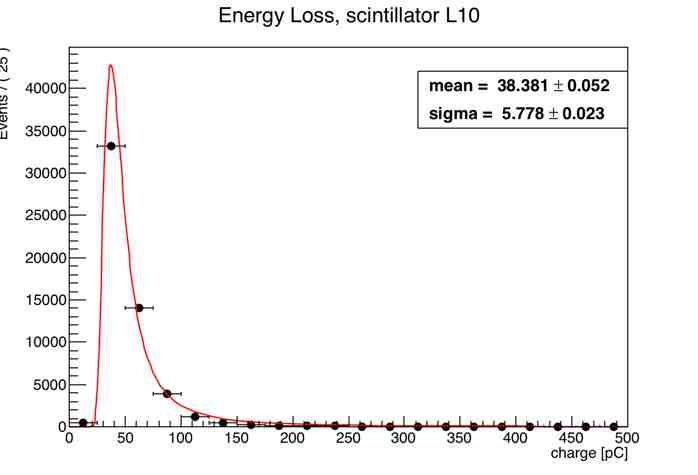
\includegraphics[width=0.8\textwidth]{plots/energy_L10.jpg}
  \caption{Curva della perdita di energia per il piano L10.}
  \label{fig:l10}
\end{figure}

\begin{figure}[H]
  \centering
  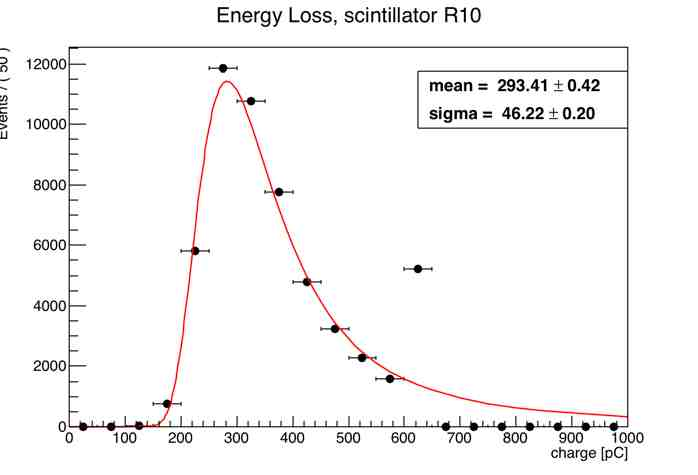
\includegraphics[width=0.8\textwidth]{plots/energy_R10.jpg}
  \caption{Curva della perdita di energia per il piano R10.}
  \label{fig:r10}
\end{figure}

\begin{figure}[H]
  \centering
  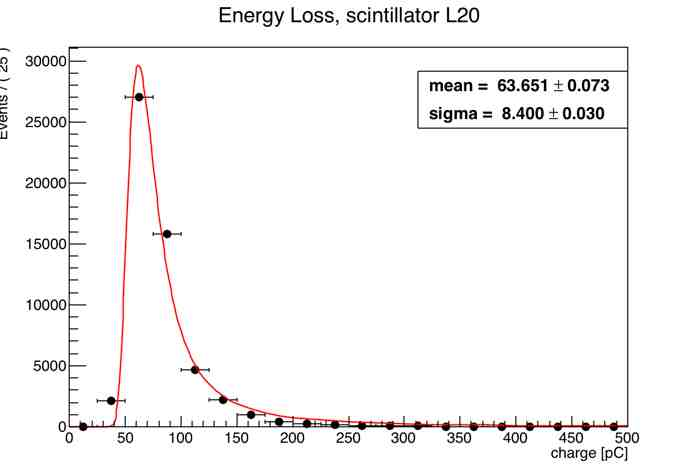
\includegraphics[width=0.8\textwidth]{plots/energy_L20.jpg}
  \caption{Curva della perdita di energia per il piano L20.}
  \label{fig:l20}
\end{figure}

\begin{figure}[H]
  \centering
  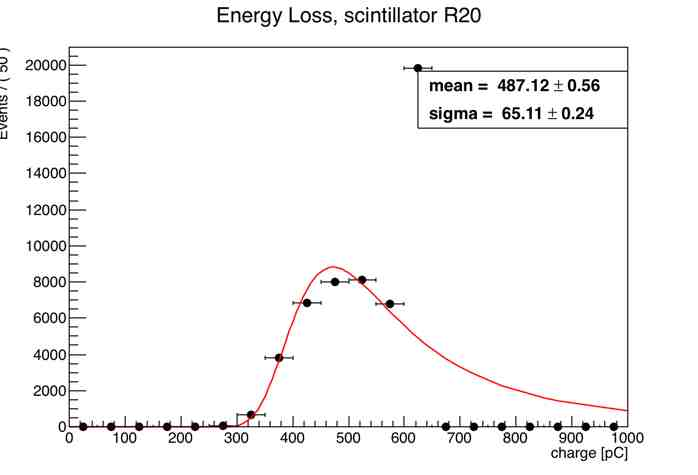
\includegraphics[width=0.8\textwidth]{plots/energy_R20.jpg}
  \caption{Curva della perdita di energia per il piano R20.}
  \label{fig:r20}
\end{figure}


\begin{thebibliography}{90}             %crea l'ambiente bibliografia
\rhead[\fancyplain{}{\bfseries \leftmark}]{\fancyplain{}{\bfseries
\thepage}}
%%%%%%%%%%%%%%%%%%%%%%%%%%%%%%%%%%%%%%%%%aggiunge la voce Bibliografia
                                        %   nell'indice
\addcontentsline{toc}{chapter}{Bibliografia}
%%%%%%%%%%%%%%%%%%%%%%%%%%%%%%%%%%%%%%%%%provare anche questo comando:
%%%%%%%%%%%\addcontentsline{toc}{chapter}{\numberline{}{Bibliografia}}
\bibitem{pdg} M. Tanabashi et al. (Particle Data Group), Phys. Rev. D 98, 030001 (2018).
\bibitem{Spurio} M. Spurio et al., Particles and Astrophysics.
\bibitem{Bendiscioli} G. Bendiscioli, Fenomeni Radioattivi.
\bibitem{Groom} D. Groom, S. Klein, Passage of particles through matter, Eur.Phys. J. C, 15: 163 (2000)
\end{thebibliography}
%%%%%%%%%%%%%%%%%%%%%%%%%%%%%%%%%%%%%%%%%non numera l'ultima pagina sinistra

